\documentclass[a4paper, 12pt]{article}
 
\usepackage[colorinlistoftodos]{todonotes}
\usepackage{setspace}

%%

\usepackage[margin=1in]{geometry} 
\usepackage{amsmath,amsthm,amssymb}

\usepackage[brazilian]{babel}
\usepackage[utf8x]{inputenc}
\usepackage{float}

\usepackage{verbatim}
\usepackage{graphicx}
 
\newcommand{\N}{\mathbb{N}} 
% indica N para números naturais
\newcommand{\Z}{\mathbb{Z}} % Z para \mathbb{Z}

\newenvironment{question}[2][Questão]{\begin{trivlist}
\item[\hskip \labelsep {\bfseries #1}\hskip \labelsep {\bfseries #2.}]}{\end{trivlist}}

\newenvironment{solving}[1][\unskip]{%
\vspace{0.2cm}

\noindent\textbf{ Solução #1.}
\vspace{0.1cm}

}
{}

% start document
\begin{document}
\newcommand{\thedepartment}{Faculdade de Engenharia Elétrica}
\newcommand{\thecourse}{FEELT}
\newcommand{\thetitle}{Temperatura, calor e primeira lei da termodinâmica}
\newcommand{\thetype}{Trabalho Extra da Disciplina de Física III}
\newcommand{\theproftitle}{Bacharel em Física}
\newcommand{\thestudent}{Lesly Viviane Montúfar Berrios\\
\centering11811ETE001}
\newcommand{\theadvisor}{Prof. Silésia Curcino}
\newcommand{\thecity}{Uberlândia}

\thispagestyle{empty}\newcommand*{\themonth}{\ifthenelse{\the\month < 2}{Janeiro }
                  {\ifthenelse{\the\month < 3}{Fevereiro }
                  {\ifthenelse{\the\month < 4}{Março }
                  {\ifthenelse{\the\month < 5}{Abril }
                  {\ifthenelse{\the\month < 6}{Maio }
                  {\ifthenelse{\the\month < 7}{Junho }
                  {\ifthenelse{\the\month < 8}{Julho }
                  {\ifthenelse{\the\month < 9}{Agosto }
                  {\ifthenelse{\the\month < 10}{Setembro }
                  {\ifthenelse{\the\month < 11}{Outubro }
                  {\ifthenelse{\the\month < 12}{Novembro }{Dezembro }}}}}}}}}}}}
                  
\begin{titlepage}
\begin{center}

	\vspace{-0.5cm}

  \begin{figure}[hbt!]
		\begin{center}
		   
\includegraphics[width=2.8cm]{ufu-logo.png}
		\end{center}
	\end{figure}
 	%\vspace{-4cm}

%\begin{doublespacing}

  \Large{\textbf{Universidade Federal de Uberlândia}}\\
  \large{\thedepartment}\\
  \large{\thecourse}\\


\vspace{5.8cm}
  \par
  \large\textbf{\thetitle}
\vspace{5.8cm} 

%\end{doublespacing}
  \par
  \thetype\\
  por\\
  %\hspace{2cm}\large{}\\

\vspace{0.8cm}
\par
  \normalsize{\thestudent}\\ [2cm]
  \theadvisor

\par\vfill
  \thecity, \themonth / \the\year

\end{center}

\end{titlepage} 
%\onehalfspacing

\begin{question}{1}  Calorimetria: estudo da troca de energia térmica.

Calcule o calor específico de um metal a partir dos dados a seguir. Um recipiente feito do metal tem uma massa de 3,6 kg e contém 14 kg de água. Um peçado de 1,8 kg do metal, inicialmente à temperatura de $180,0^{\circ}C$, é mergulhado na água. O recipiente e a água estão inicialmente a uma temperatura de  $16,0^{\circ}C$ e a temperatura final do sistema (termicamente isolado) é  $18,0^{\circ}C$. $c_a=4,18KJ/Kg.K$.

\end{question}

\begin{solving}
Para o Equilíbrio térmico tem-se que na troca de calor $\sum Q = 0$. Logo, como o sistema é termicamente isolado é válida a relação:
$$Q_{recipiente} + Q_{agua}+Q_{pedaco}=0$$

Portanto, 
\begin{gather*}
m_{recipiente} c_{metal}\Delta T_{recipiente} + m_{agua} c_{agua}\Delta T_{recipiente} + m_{pedaco} c_{metal}\Delta T_{pedaco} = 0\\
 c_{metal}\, (m_{recipiente}\Delta T_{recipiente}+ m_{metal} \Delta T_{pedaco}) = -m_{agua} c_{agua}\Delta T_{recipiente}\\
 c_{metal} = -\dfrac{m_{agua} c_{agua}\Delta T_{recipiente}}{m_{recipiente}\Delta T_{recipiente}+ m_{metal} \Delta T_{pedaco}}
\end{gather*}

Substituindo com os dados do exercício:
\begin{gather*}
c_{metal} = -\dfrac{14\cdot (4,18)\cdot 2}{(3,6)\cdot 2+ (1,8)\cdot (18-180)}\\
c_{metal} = 0,4115\, KJ/Kg.K\\
\text{ou}\\
c_{metal} = 0,0985\, cal/g^{\circ}C
\end{gather*}

\end{solving}

\vspace{0.3cm}
\begin{question}{2} Calor e Trabalho.

Um gás em uma câmara fechada passa pelo ciclo mostrado na Figura \ref{fig1}. Determine a energia transferida pelo sistema na forma de calor durate o processo $CA$ se a energia adicionada como calor $Q_{AB}$ durante o processo $AB$ é $20,0J$. Nenhuma energia é transferida como calor durante o processo $BC$ e o trabalho realizado durante o ciclo é $15,0J$.

\begin{figure}[!htb]
\centering
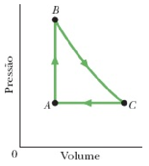
\includegraphics{Q2}
\caption{Ciclo de um gás em uma câmara fechada.}
\label{fig1}
\end{figure}
\end{question}
 
\begin{solving}
Como o gás passa por um processo cíclico, tem-se que, após certas trocas de calor e de trabalho, o sistema volta ao estado inicial. Nesse caso, nenhuma propriedade intrínseca do sistema varia, incluindo a energia interna $\Delta E_{int}$. Assim, da Primeira Lei da Termodinâmica, $\Delta E_{int}=Q-W \Rightarrow Q=W$ .

Logo,  $Q_{AB} + Q_{BC} + Q_{CA}= W_{tot}$.
\begin{gather*}
20 + 0 + Q_{CA}= 15\\
Q_{CA} = -5J
\end{gather*}
\end{solving}

\begin{question}{3} Mecanismos de Transferência de Calor: Radiação.

\emph{Aglomerações de pinguins.} Para suportar o frio da Antártica, os pinguins-imperadores se aglomeram em bandos. Suponha que um pinguim pode ser modelado por um cilindro circular de altura $h=1,1m$ e com uma área da base $a=0,34m^2$. Seja $P_i$ a taxa com a qual um pinguim isolado irradia a energia para o ambiene (pelas superfícies superior e lateral); nesse caso, $NP_{i}$ é a taxa com a qual $N$ pinguins iguais e separados irradiam energia. Se os pinguins se aglomeram para formar um \emph{cilindro único} de altura $h$ e área da base $N\cdot a$, o cilindro irradia a uma taxa $P_{u}$. Se $N=1000$, determine (a) o valor da razão $P_{u}/NP_{i}$ e (b) a redução percentual da perda de energia devido à aglomeração.
\end{question}

\begin{solving}
Quando um sistema e o ambiente trocam energia por meio de ondas eletromagnéticas, diz-se que essas ondas são \emph{radiações térmicas}. Assim, a taxa $P_{rad}$ com a qual um objeto emite energia por radiação eletromagnética é dada por $P_{rad}=\sigma \varepsilon A\, T^{4}$, em que $\sigma=5,6704 \times 10^{-8} W/m^2\cdot K^4$ (\emph{constante de Stefan-Boltzmann}) e $\varepsilon \in (0,1)$ é a \emph{emissividade} da superfície do objeto.
\vspace{0.3cm}

\noindent (a) Razão $P_{u}/NP_{i}$:

Sabendo-se que a área de radiação para um pinguim é dada como $A_{i}=a+h\cdot 2\sqrt{\pi a}$, e para $N$ pinguins como $A_{u}=N\cdot a+h\cdot 2 \sqrt{\pi N\cdot a}$, tem-se:

\begin{gather*}
\dfrac{P_{u}}{NP_{i}}= \dfrac{\sigma \varepsilon A_u}{N\, \sigma \varepsilon A_i\, T^{4} }\\
\dfrac{P_{u}}{NP_{i}}= \dfrac{A_u}{N\cdot A_i}\\
\dfrac{P_{u}}{NP_{i}}= \dfrac{N\cdot a+h\cdot 2 \sqrt{\pi N\cdot a}}{N\cdot (a+h\cdot 2\sqrt{\pi a})}\\
\dfrac{P_{u}}{NP_{i}}= \dfrac{1000\cdot 0,34+1,1\cdot 2 \sqrt{\pi 1000\cdot 0,34}}{1000\cdot (0,34+1,1\cdot 2\sqrt{\pi 0,34})}\\
\dfrac{P_{u}}{NP_{i}}\approx 0,1576
\end{gather*}
\vspace{0.3cm}

\noindent (b) Redução percentual da perda de energia devido à aglomeração:

Como $P_{u}\approx 0,1576\cdot NP_{i}$, tem-se a redução de perda de energia de $100\%-15,76\%=84,24\%$, quando os pinguins estão aglomerados.
\end{solving}

\end{document}